\documentclass[]{article}
\usepackage[a4paper, total={6in, 8in}]{geometry}
\usepackage{pdflscape}
\usepackage{booktabs}
\usepackage{multicol}
\usepackage{mathtools, amssymb, amsmath}
\usepackage[
  sorting=none,
  sortcites=true,
  backend=bibtex,
  giveninits=true,
  style=authoryear-comp,
  natbib=true,
  maxcitenames=2,
]{biblatex}
\bibliography{bibliography}

\newcommand{\todo}[1]{{\color{red}[\textit{TODO: #1}]}}

\makeatletter
\newcommand{\citetnl}[1]{%
  \@firstofone{\citet{#1}}}
\makeatother

\usepackage{tikz}
\usetikzlibrary{calc}
\usetikzlibrary{shapes.geometric, arrows, fit}

\tikzstyle{process} = [rectangle, 
minimum width=12cm, 
minimum height=1cm, 
text width=11cm, 
draw=black, 
fill=white,
rounded corners]

\tikzstyle{subprocess} = [rectangle, 
minimum width=5cm, 
minimum height=0.6cm, 
text centered, 
text width=5cm, 
draw=black, 
fill=white]

\tikzstyle{lsnode} = [rectangle, 
minimum width=2cm, 
minimum height=0.6cm, 
text centered, 
text width=2cm, 
draw=black, 
fill=white]

\tikzstyle{arrow} = [thick,->,>=stealth]
\tikzstyle{dashedarrow} = [dashed,->,>=stealth]

\title{Integrated Vehicle and Crew Scheduling for Electric Buses with Realistic Charging Behavior}
\date{July 2025}
\author{Thomas van der Plas, Han Hoogeveen, Philip de Bruin}
\begin{document}
\maketitle

\section{Introduction}
Electric vehicles are beginning to make up large portions of the fleet for
public transport providers. In The Netherlands for instance, around 21\% of all
registered buses are already electric according to the \citet{RDW}. However,
in order to meet \citet{europaRegulation20181999} on climate and sustainability, individual
line operators such as the Dutch \citet{qbuzzQbuzz} are slowly replacing even more of their old
combustion based fleet with electric vehicles. It is therefore almost certain that this share will only grow in
coming years across different countries. \\
This shift in energy source has introduced new challenges to the methods currently in use to keep our public transport moving. Of primary concern are charging infrastructure and vehicle ranges, both of which are much more limited than their traditional combustion based counterparts. The planning process which has traditionally been used, as outlined in Figure \ref{fig:planning-overview}, therefore requires additional research into each of its steps in order to incorporate these newly relevant constraints.\\
\noindent In this work, we will focus on incorporating electric vehicle restrictions into two of these steps: vehicle scheduling and crew scheduling. Specifically, we will consider the scheduling of electric buses and their drivers, as these two steps make up a majority of day-to-day costs within the bus transit sector. \\
\begin{figure}[ht]
  \centering
  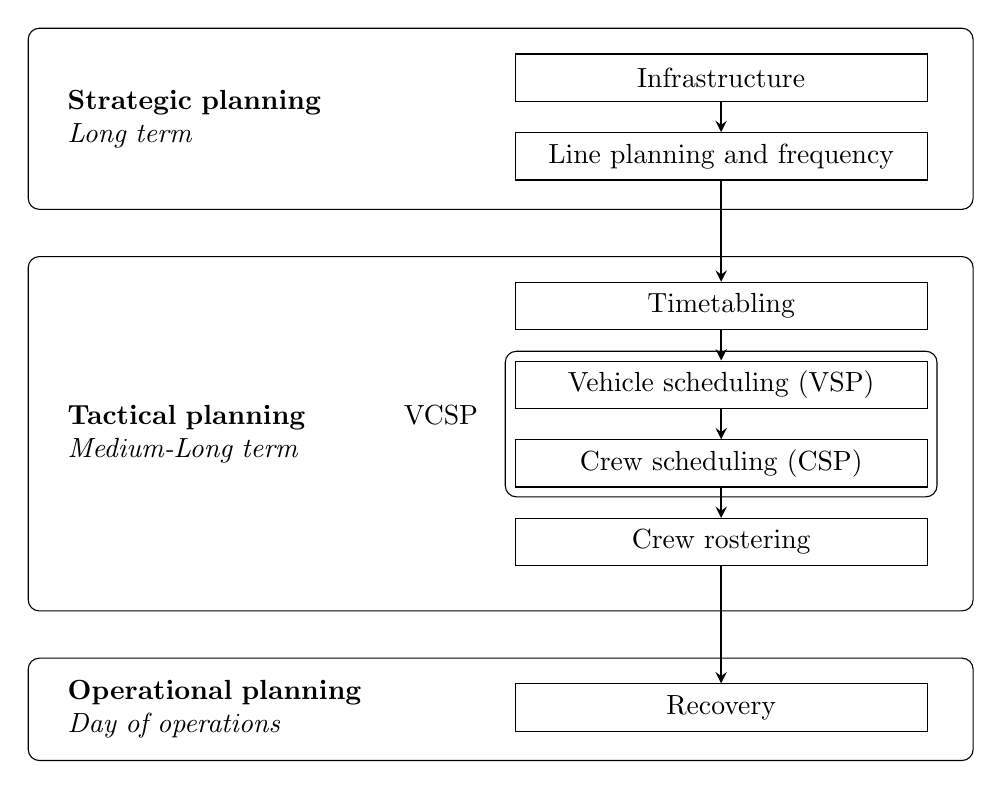
\begin{tikzpicture}[node distance=2cm]
    \node (strategic) [process, minimum height=2.3cm] {\textbf{Strategic planning}\\\textit{Long term}};
    \node at (strategic.base) (infra) [subprocess, xshift=2.8cm, yshift=0.4cm] {Infrastructure};
    \node at (strategic.base) (line) [subprocess, below of=infra, yshift=1cm] {Line planning and frequency};

    \node (tactical) [process, minimum height=4.5cm, below of=strategic, yshift=-2cm] {\textbf{Tactical planning}\\\textit{Medium-Long term}};
    \node at (tactical.base) (timetable) [subprocess, xshift=2.8cm, yshift=1.5cm] {Timetabling};
    \node at (tactical.base) (vehicle) [subprocess, below of=timetable, yshift=1cm] {Vehicle scheduling (VSP)};
    \node at (tactical.base) (crew) [subprocess, below of=vehicle, yshift=1cm] {Crew scheduling (CSP)};
    \node at (tactical.base) (VCSP) [rounded corners, draw=black, fit=(vehicle) (crew), align=left] {\hspace{-4em}VCSP};
    \node at (tactical.base) (rostering) [subprocess, below of=crew, yshift=1cm] {Crew rostering};

    \node (operational) [process, minimum height=1.3cm, below of=tactical, yshift=-1.5cm] {\textbf{Operational planning}\\\textit{Day of operations}};
    \node at (operational.base) (recovery) [subprocess, xshift=2.8cm, yshift=-0.1cm] {Recovery};

    \draw [arrow] (infra) -- (line);
    \draw [arrow] (line) -- (timetable);
    \draw [arrow] (timetable) -- (vehicle);
    \draw [arrow] (vehicle) -- (crew);
    \draw [arrow] (crew) -- (rostering);
    \draw [arrow] (rostering) -- (recovery);
  \end{tikzpicture}
  \caption{A general overview of the public transport planning process, based on \citet{Ceder1986, Ibarra-Rojas2015, Perumal2022LitRev}.}
  \label{fig:planning-overview}
\end{figure}
The goal of vehicle scheduling is generally to assign vehicles such that a set of trips is covered. In the case of buses, trips are given by the timetables for the individual routes as generated in the previous planning step. Our goal is therefore to assign sequences of compatible trips to buses such that each individual trip is driven. \\
In order to do this, a collection of vehicle tasks must be generated. A vehicle task can be seen as the individual schedule that a bus will follow throughout the day: it may start at a bus storage facility (more commonly called a depot), then perform one or more trips, before finally returning to the depot. The driving actions performed between between a depot and a trip, as well as those between trips themselves are called deadheads. The costs of driven deadheads along with the total number of buses used are the main focus for minimization, as the costs incurred for driving the trips themselves are fixed. This cost minimization problem is often referred to as the vehicle scheduling problem or VSP. The single-depot VSP with a single vehicle type is solvable in polynomial time, however extensions such as multiple vehicle types or limited vehicle ranges are shown to be NP-Hard by \citet{Bunte2009} and \citet{Haghani2002} respectively. \\
Once vehicle tasks are known, we can move on to scheduling our crew. Here, our goal is to find an assignment of crew members to vehicles  such that the previously made vehicle tasks can actually be performed. Continuing within the context of bus planning, we now need to match drivers with our previously planned buses such that there is always a driver present while the bus is moving. In order to do this, a set of crew tasks must be created that completely cover the given vehicle tasks. \\ 
A one-to-one mapping between crew tasks and vehicle tasks is not always possible; overall driving time for a driver is limited in a single day due to labor regulations, and for longer shifts breaks are mandatory as well. As vehicles don't have these constraints, a vehicle task may not be feasible to perform in its entirety for a single driver. It is therefore necessary to split vehicle tasks up into multiple segments, whereafter we can create crew tasks that consist of a sequence of one or more compatible segments. The costs of vehicle tasks themselves are fixed as they must always be driven; in order to minimize costs, we must therefore find a covering set of crew tasks which minimizes the number of required crew members and paid hours in which the driver is not actively driving. This minimization problem is referred to as the crew scheduling problem or CSP, and has been shown to be NP-Hard by \citet{Fischetti1989}. \\ 
Crew scheduling is the greatest contributor to day-to-day costs; a recent estimate by \citet{Perumal2019Crew} puts it at around 60\% of the overall operational costs for bus transit providers in Northern Europe. As can be seen however, the VSP and CSP are very closely related. The vehicle tasks that are selected in the VSP directly determine what crew
tasks are feasible within the CSP. It is therefore not always optimal to
fully minimize costs in the vehicle scheduling process, as this might incur
higher overall costs due to crew scheduling. We can therefore roughly split the
solving of vehicle and crew assignments into two separate approaches:
sequential, in which the VSP and CSP are solved separately; or integrated, in
which the VSP and CSP are solved such that overall costs are minimized
simultaneously. The integrated approach is often referred to as the vehicle and
crew scheduling problem, or VCSP. \\
A lot of work has already been done for the VSP, CSP and VCSP.
Both the sequential and integrated approach have been extensively studied since the 1980s, as shown by surveys such as \citet{Bodin1983}. The introduction of electric vehicles has however introduced significant constraints on charging and vehicle ranges, invalidating a formerly often made assumption that a vehicle was able to drive an entire day without being refueled. This most directly effects the VSP, as charging periods now need to be added throughout the day in order to
effectively use buses. The version of the vehicle scheduling problem which incorporates these constraints, referred to as the
E-VSP, has been the focus of many studies going back to around 2014. We refer the reader
to a survey by \citet{Perumal2022LitRev} for a detailed overview of recent progress. \\
Limited literature does exist on the integrated VCSP with electric vehicles (E-VCSP), however
simplifying assumptions are made which might limit real world applicability or
accurate modeling of costs. Most notably, assumptions are currently made about charging
locations (such as only being able to charge at a bus depot) or charging
behavior (such as modeling the process as being purely linear or only allowing
full charges). Additionally, to the best of our knowledge battery degradation
due to usage patterns has not been included in any integrated models at the
time of writing. Our aim is to introduce an integrated E-VCSP model which incorporates more realistic behavior for battery charging and usage, by including the following:
\begin{itemize}
  \item Nonlinear battery charging times.
  \item Cost of battery degradation due to usage patterns.
  \item Capacitated charging stations at both depots and the endpoints of a trip.
  \item Partial charging of the battery throughout the day.
\end{itemize}
Using this model, we compare the overall costs of the integrated approach to an equivalent sequential formulation using instances provided by Qbuzz. \todo{Alleen kosten vergelijken lijkt me met minimale doel; Het liefst zou ik ook nog iets van gevoeligheidsanalyse doen voor invloed van oplaadlocaties/batterijcapaciteit/etc, maar dat is afhankelijk van hoeveel tijd het model werkend krijgen kost}. \\  
This work is organized as follows. In Section 2, we will discuss work related to the E-VCSP and give an overview of common ways of modeling and solving the problem. In Section 3, we give our formal problem definition.\ \todo{Meer secties}.

% We will now give an informal overview of the
% problems at hand. A more formal definition can be found in Section
% \ref{sec:problem_def} \todo{work in progress}. \\
% The Vehicle Scheduling Problem (VSP) aims to find a set
% of minimum cost vehicle tasks such that all trips that need to be driven
% throughout a time period are covered. In this, a trip is defined as full or
% partial travel of a vehicle along a predetermined route, and a vehicle task is
% defined as a set of sequential operations that a vehicle will perform. A task for a
% vehicle must start at a depot, perform a number of compatible trips (that is,
% trips which can be performed sequentially while respecting driving times
% between trips), before finally returning to its original depot. In order to
% minimize operational costs, both the number of used vehicles and the overall driven
% distance between trips need to be minimized. \\ The VSP
% with a single depot and unconstrained vehicle ranges can be solved in
% polynomial time \citet{Freling2003SDVSP}. The multi-depot variant of the problem
% on the other hand is known to be NP-Hard, and the addition of constrained vehicle ranges such as those found
% in EVs also make the problem NP-Hard \citet{Bodin1983}. We will consider a
% general depot case with constrained vehicle ranges due to the inclusion of EVs,
% and will therefore refer to the VSP as being NP-Hard. \\\\ The Crew
% Scheduling Problem (CSP) on the other hand aims to find a minimum cost
% assignment of crew members to vehicle tasks. Given a set of vehicle tasks and
% crew members, the goal is to find an assignment of crew members such that each
% vehicle is always driven by at least one driver. In this, constraints such as
% maximum working time on a day, driver breaks and handovers between different
% drivers on the same vehicle need to be considered. The primary goal for
% minimization here is the total number of workers needed and hours worked. The
% CSP is also known to be an NP-Hard problem \citet{Fischetti1989}.\\\\ As can be seen, the VSP and CSP are closely related.  

\begin{table}
  \centering
  \begin{tabular}{ll}
    \toprule
    \multicolumn{1}{l}{\textbf{Abbreviation}} & \multicolumn{1}{l}{\textbf{Definition}}               \\
    \cmidrule(lr){1-1}\cmidrule(lr){2-2}
    ALNS                                      & Adaptive Large Neighborhood Search                   \\
    B\&P                                      & Branch-and-Price                                      \\
    CG                                        & Column Generation                                     \\
    CP                                        & Constraint Programming                                \\
    CSP                                       & Crew Scheduling Problem                               \\
    E-\dots                                   & Problem \dots with electric vehicles                  \\
    LNS                                       & Large Neighborhood Search                            \\
    LS                                        & Local Search                                          \\
    MDVSP                                     & Multi Depot Vehicle Scheduling Problem                \\
    MIP                                       & Mixed Integer Program                                 \\
    SAA                                       & Simulated Annealing Algorithm                         \\
    SDVSP                                     & Single Depot Vehicle Scheduling Problem               \\
    SoC                                       & State of Charge                                       \\
    TCO                                       & Total Cost of Ownership                               \\
    ToU                                       & Time of Usage                                         \\
    TVSP                                      & Integrated Timetabling and Vehicle Scheduling Problem \\
    VCSP                                      & Integrated Vehicle and Crew Scheduling Problem        \\
    VSP                                       & Vehicle Scheduling Problem                            \\
    \bottomrule
  \end{tabular}
  \label{tab:nomenclature}
  \caption{Nomenclature used in this work}
\end{table}

\section{Related work}
In this section, we will discuss work related to our research into the E-VCSP. An overview of the nomenclature used has been included in Table \ref{tab:nomenclature}, and an summary of how batteries and charging behavior is modeled in the discussed works has been included in Table \ref{tab:eVCSP-lit}.
\begin{landscape}
\null
\vfill
\begin{table}[h]
  \centering
  \begin{tabular}{llllllll}
    \toprule
                                     & Model   & ToU & SoC & Nonlinear Ch. & Partial Ch. & Ch. Location & Degradation \\
    \cmidrule(lr){2-8}
    \citet{Li2014}               & E-VSP   & No  & D   & No            & No          & D            & No          \\
    \citet{vanKootenNiekerk2017} & E-VSP   & Yes & C/D & Yes           & Yes         & D/T          & Yes         \\
    \citet{Olsen2020}            & E-VSP   & No  & C   & Yes           & Yes         & D/T          & No          \\
    \citet{Zhang2021}            & E-VSP   & No  & C/D & Yes           & Yes         & D            & Yes         \\
    \citet{Parmentier2023}       & E-VSP   & No  & C   & Yes           & Yes         & D/T          & No          \\
    % \citet{Pulyassary2024}       & E-VSP   & No  & C/D & Yes           & Yes         & T            & No          \\
    \citet{deVos2024}            & E-VSP   & No  & D   & Yes           & Yes         & D/T          & No          \\
    \addlinespace[0.4em]
    \citet{Perumal2021}          & E-VCSP  & No  & C   & No            & No          & D            & No          \\
    \citet{Wang2022}             & E-VCSP  & Yes & C   & No            & Yes         & D            & No          \\
    \citet{Sistig2023}           & E-VCSP  & No  & C   & No            & Yes         & D/T          & No          \\
    \citet{Shen2023}             & E-VCSP  & No  & C   & No            & No          & D/T          & No          \\
    \citet{Cong2024}             & E-VCSP  & Yes & C   & No            & Yes         & D            & No          \\
    \addlinespace[0.4em]
    \citet{Ham2021}              & E-VRPTW & Yes & C   & No            & Yes         & D            & No          \\
    \citet{Stadnichuk2024}       & E-TVSP  & No  & C   & No            & Yes         & D/T          & No          \\
    \bottomrule
  \end{tabular}
  \caption{A brief overview of battery modeling in E-VCSP related literature. SoC modeled as (D)iscrete or (C)ontinuous variable, Charge locations at (D)epot or (T)erminal trip stops, Degradation of battery in cost function}
  \label{tab:eVCSP-lit}
\end{table}
\vfill
\end{landscape}

\todo{uitleg van de SDVSP}
\subsection{(E-)VSP}
Before considering previous work on the E-VSP, we will first cover the most basic form of vehicle scheduling: that which only considers a single depot, single vehicle type and unlimited vehicle ranges. This problem, referred to as the single depot vehicle scheduling problem (SDVSP), forms the underlying basis of both the multi-depot and electric vehicle extensions that we will consider later. We will therefore give a brief summary of one the most common models and solution methods used for the SDVSP, thereby having a baseline to which we can compare extensions. For a more comprehensive overview on different models used for the SDVSP and multi-depot VSP (MDVSP), we refer the reader to a review by \citet{Bunte2009}. \\
As mentioned before, our goal in the SDVSP is to create a set of vehicle tasks throughout the day in which the number of vehicles and the cost of driven deadheads is minimized while covering all trips. In order to solve this problem, a graph consisting of the trips and depot can be created. In this graph, we can then solve a min-cost flow problem in which all trips are covered; the optimal vehicle tasks then follow from the flow paths along the trips. \\
More formally, given a set of trips $T$ and a single depot $d$, a graph $G = (V, A)$ can be constructed. Let $V = \{ v^s_t \mid t \in T \} \cup \{ v^e_t \mid t \in T \} \cup \{ v^s_d, v^e_d \}$, in which each pair of nodes $(v^s_t, v^e_t)$ represent the start and end of trip $t$ respectively. Additionally, the pair of nodes $(v^s_d, v^e_d)$ represent the depot at the start and end of the day. Next, let $A_T = \{ (v^s_t, v^e_t) \mid t \in T \}$ represent the arcs connecting the start and end of the trip, each with cost equal to the cost of driving the trip. Let $A_{DH} = \{ ( v^e_t,\: v^s_{t'}) \mid (t, t') \in T \times T,\: t'\text{ can be driven after }t \}$ represent a set of arcs which model feasible deadhead trips; once again, each with cost equal to those incurred when driving the deadhead between $t$ and $t'$. Let $A_{D} = \{ (v^s_d, v^s_t) \mid t \in T \} \cup \{ (v^e_t, v_d^e) \mid t \in T \}$ represent deadheads from the depot to a trip and vice versa, once again with costs equal to those when driving the deadheads. If fixed costs per vehicle are required, these can be added to arcs leaving the depot. Finally, let $A = A_T \cup A_{DH} \cup A_D$, and let all arcs have capacity equal to 1. \\
Setting $v^s_d$ as our source and $v_d^e$ as our sink, we can now find a min-cost max-flow across the graph $G$. Due to our construction, all trips must be covered by exactly 1 flow, resulting in flow paths which we can directly use as vehicle tasks due to the assumption that our vehicles have enough range. It is therefore also shown that the SDVSP can be solved in polynomial time, as polynomial time min-cost max-flow algorithms exist and the graph elements are of size $|V| = O(|T|)$ and $|A| = O(|T|^2)$.\\
Two common extensions to the problem make it NP-Hard: the inclusion of multiple vehicle types, as well the use of multiple depots under the assumption that vehicles must return to their depot of origin. Both of these extensions are also discussed in \citet{Bunte2009}. The modification to the SDVSP flow network is the same in either case: an additional source/sink pair can be added for each new depot or vehicle type, and connected to the trips in the same way as the original depot. The problem then turns into into an integral multi-commodity flow, which has been shown to be NP-Hard by \citet{Even1975}. \\
The introduction of any resource constraints within the VSP has also been shown to be NP-Hard by
\citet{Bodin1983}. The E-VSP specifically deals with constraints on the driving range of vehicles, thereby making it closely related to the vehicle scheduling problem with route time constraints (VSP-RTC) as described by \citet{Haghani2002}. The key difference between these two problems is that the
E-VSP allows for (partial) recharging of a vehicle throughout the operating
period, whereas the VSP-RTC assumes a fixed maximum travel time for the
vehicle within the given period. The E-VSP has been shown to be NP-Hard by \citet{Sassi2014}. \\\\
\citet{Li2014} was one of the first to consider a solution method for the E-VSP. A single-depot case with a single vehicle type is considered, in which the assumption is made that recharging (or battery swaps) can be performed in a fixed 5-minute window. The model is based on an extension of the SDVSP network, with the inclusion of total driving time constraints. Additionally, extra time-discretized nodes are added to represent capacitated battery charging/swap stations. For smaller instances, the model can be solved to optimality using column generation and branch-and-price (B\&P). For larger instances, an alternate approach using truncated column generation followed by a local search to find a local
optimum is used instead. The proposed methods are tested on trips in the San Francisco Bay
Area, with a maximum instance size of 242 trips. These tests resulted in
optimality gaps of $<5\%$ for buses able to drive 150km, and between 7-15\%
for a range of 120km depending on the instance. \\
\citetnl{vanKootenNiekerk2017} introduces two models which aim to solve the single depot E-VSP
while taking into account time dependent energy prices (ToU pricing), nonlinear charging times and
battery degradation due to depth of discharge. The first model only allows for linear charging and no consideration for degradation or ToU, but uses continuous state of charge (SoC) variables which are added to the SDVSP network. The second model does allow for the extra inclusions, achieving this by duplicating trip nodes in the SDVSP network for discrete SoC values. The second model is solved using column generation and lagrangian relaxation, resulting in a possibly non-optimal solution. Tests are performed using data provided by Belgian bus company De Lijn in the city Leuven, using a total of 543 trips. They show that the
discretized model can be solved in a considerably shorter time frame for large instances with similar results to
the continuous model. \\
\todo{langer!}
\citet{Olsen2020} introduce a solution to the E-VSP which models the nonlinear phase of charging as an exponential function. They focus on showing that a (piecewise) linear approximation for the second phase of charging can misrepresent the SoC and required charging times. \\
\citet{Zhang2021} apply a similar method to the one found in \Citet{vanKootenNiekerk2017}. They consider a single depot with capacitated charging infrastructure,
with multiple round trip lines originating from the depot. In addition to this, they also incorporate nonlinear charging behavior and battery depreciation using discrete SoC and time nodes in the SDVSP network. They solve using a combination of CG and B\&P. Tests are done on both randomly generated instances as well as 6 not yet electrified lines with up to 160 and 197 trips
respectively.\\
\citet{Parmentier2023} consider a scalable approach to the E-VSP with non-linear charging. They introduce the concept of nondominated charging arcs, which are represented as deadhead arcs within the SDVSP. Their use considerably reduces the amount of candidate charging arcs when multiple charging points are available, as an arc is only considered if there is not another arc available with higher resulting charge and lower cost. In order to solve, a combination of CG and B\&P techniques are used. A more computationally efficient version of the pricing problem is also provided by the nondominated charging arcs when charging
infrastructure is uniform. Testing is done on the \textit{large}
instances introduced by \citet{Wen2016} which included up to 8
depots, 16 charging stations and 500 trips. Here, they are able to find
solutions that only have an 0.06\% optimality gap. \\
% \citet{Pulyassary2024} show that the single depot E-VSP is solvable in polynomial time given the
% assumption that the shortest path between two trips in the flow network is
% equal to the path with lowest battery usage. They
% consider the case in which charging at a select number of capacity bound nodes
% is allowed with nonlinear charging behavior. For the single depot case, a
% $O^*(|T|^6)$ algorithm for finding a set of vehicle schedules with lowest cost
% given trips $T$ is provided based on DP. Additionally, polynomial algorithms
% for determining maximum feasible charging capacity and minimum-cost flows based
% on LP are provided. No computational experiments are performed. \\\\
\citet{deVos2024} consider the E-VSP with partial recharges and capacitated charging stations. Their model includes discrete SoC trip nodes and discrete SoC and time charging location nodes, similar to the model found in \citet{Zhang2021}. Using these, a primal network is created using pessimistic SoC rounding when connecting trips with feasible deadheads. In order to solve, they apply CG with two separate approaches:
branch-and-price and a diving heuristic. To overcome the limitations of dual
bounds resulting from a discretized model, they incorporate ideas from \citet{Boland2017} resulting in a dual network with optimistic connections. This gives the same bounds as the ones found in the
non-discretized model. Testing is performed on a bus concession south of
Amsterdam with 816 trips, with subsets being used as smaller instances.
Optimality gaps of 1.5-2.7\% are achieved across instances. They additionally
note that the framework as provided can easily be extended for nonlinear
charging functions and depth-of-discharge battery degradation. 

\subsection{CSP}
Given a solution to the (E-)VSP, the corresponding CSP is most often solved as a set partitioning (or set covering) problem. Here, the tasks described by the sequences of trips generated during vehicle scheduling must be covered by the individual schedules of crew members. This problem has been shown to be NP-Hard in general by \citet{Fischetti1989}.\\
Research into this subject is primarily done in the context of airline crew planning; crew costs in this field are generally even higher than those found in the more general public transport sector, as shown in \citet{Barnhart2003}. Additionally, strong labor unions and restrictive labor legislation due to safety concerns cause a large number of constraints to be applied to crew schedules, resulting in a non-trivial problem to solve. \\
Results achieved in the aviation space quite easily generalize to other sectors, and we therefore refer the reader to a recent review by \citet{Deveci2018} for an overview of the state of the art. 

\subsection{(E-)VCSP}
The VCSP has been a widely studied problem. Following the call for integrated methods by \citet{Bodin1983} and others in the 1980s, a large number of different methods has been applied to integrate the VSP and CSP. We refer the reader to a recent review by \citet{Ge2024} for a more general overview of work done in the field in the past years. \\
One work that we will individually highlight is that of \citet{Huisman2005}, due to its use of Lagrangian relaxation to connect the VSP and CSP . For readers unfamiliar with the technique, we recommend an introduction by \citet{Beasley1993}. Huisman et al. consider the multi-depot variant, and use a combination of CG and Lagrangian relaxation to solve both the MDVSP as well as the connection with the CSP. Of note is their assumption that crew members from each individual depot are only allowed to work on trips connected to said depot, allowing for individual depot CSPs to be solved as a subproblem. They test on instances in the Randstad metro area in the Netherlands with a maximum of 653 trips and 4 depots. \\\\
As for the electric counterpart of the VCSP, at time of writing we are aware of only five other works that discuss the integrated variant. \\
\citet{Perumal2021} were the first to offer a solution to the E-VCSP. They consider an instance of the problem in which only full recharges at the depot with a fixed duration of
120 minutes are possible. In order to solve, an ALNS was introduced which incorporates a B\&P heuristic
which has been previously used to solve the MDVSP, E-VSP and VCSP. The authors tested using real life data from lines in Denmark and Sweden with a
maximum instance size of 1109 trips and multiple depots, and report an improvement of $1.17-4.37\%$
across different instances when compared to a sequential approach. \\
\citet{Wang2022} introduce a two layered model using particle swarms and an
$\epsilon$-constraint based mechanism which allows for a mix of traditional
combustion and electric buses. The model incorporates partial
depot charging, as well as measures to ensure that crew is primarily assigned
to the same vehicle throughout the day. A circular bus route with a single
depot in Changchun, China with 68 daily trips is used as a basis for testing,
with a focus on electric versus diesel usage and driver satisfaction. \\
\citet{Sistig2023} also offered an ALNS based approach, which aimed to
improve upon the approach presented by \citet{Perumal2021} by including partial
recharges, opportunistic charging at terminal stops of trips and non-fixed
ranges for the vehicles. In order to solve, they implement a
selection of 3-step ALNS neighborhoods consisting of E-VSP modification,
finding a solution to the corresponding CSP and consequently modifying the CSP
solution. Tests were done using an instance of a city route in Germany, with a
single depot and a total of 282 trips. Different scenarios based on possible
crew break and relief locations were considered in order to compare diesel and
electric TCO. Additionally, sensitivity analysis of the TCO was done for
parameters such as costs for electricity and drivers. \\
\citet{Shen2023} provide a minimum-cost flow framework for the E-VSP which is
integrated with a set partitioning based approach for the E-CSP. They only provide full recharge capabilities at the depot,
however focus on the inclusion of a distinction between energy use when driving
and standing still in order to more accurately model real life traffic. A city
line in China with 270 daily trips and a single depot is used for testing,
resulting in cost savings of up to 8.7\% when compared to a sequential
approach. \\
\citet{Cong2024} provide a hybrid MIP and SAA based approach to optimizing a mixed
fleet of combustion and electric vehicles with ToU electricity pricing. In each SAA iteration, a collection of new E-VSP trip
assignments are created using neighborhood operations, after which two MIP
models are sequentially employed to solve for charging and crew schedules. The
methods are tested on a collection of 3 bus routes originating from the same
depot in Changchun City, China with a total of 520 trips across all routes.
When compared to the sequential approach, the integrated vehicle schedule was
able to reduce costs by 0.8\%. 

\subsection{Other related fields}
The VSP is closely related to the vehicle routing problem (VRP); in this problem, the aim is to find minimum cost routes for vehicles originating from a depot and needing to pass multiple stops, most commonly for pickup or delivery with capacity constraints. The extension of the E-VRP which includes arrival time windows (E-VRPTW) is most closely related to the E-VSP, as the use of 0-width windows allows us to define the same precedence constraints as those naturally defined by trips in the VSP. \\
An example of work done on the E-VRPTW is that of \citet{Ham2021}. They consider a single depot case in which they model ToU pricing and partial recharges during delivery routes. In order to model costs, a lexicographical minimization is done over the number of vehicles used, total distance traveled and energy recharged. In order to solve, a hybrid MIP and CP algorithm is used in which CP is used to model ToU related variables, and MIP is used to model the rest of the constraints. \\\\
Research has also been done into integrating the E-VSP with the step before it in the planning sequence: timetable planning. This problem, the E-TVSP, has recently been studied in the work of \citet{Stadnichuk2024}. They allowed results of the E-VSP to introduce optimality cuts into the MIP used for creating timetable plans, thereby reducing overall cost. This is achieved by transforming the E-VSP problem into one of bin packing with conflicts, after which three different heuristic methods are applied and compared. They additionally prove that the bounds of the used heuristics are tight for their given instances. 

\section{Problem definition}
\label{sec:problem_def}
In this section, we will give a formal definition of the integrated electric vehicle and crew scheduling problem (E-VCSP). We will begin with a model which does not consider capacitated charging stations. \\
Let us start by formally defining a feasible vehicle task $v$ for a vehicle of type $\rho$. A vehicle task, as mentioned before, must start at a depot, then perform a sequence of compatible trips, before finally returning to the same depot. During this sequence, the SoC $\sigma$ of the vehicle must always satisfy $\sigma^\rho_{min} \leq \sigma \leq \sigma^\rho_{max}$, ensuring that the battery capacity for the vehicle type is not violated. A vehicle task can therefore be defined as a sequence of steps $S = \{ s_0, s_1, \dots, s_n, s_{n+1} \}$, where $s_0 = s_{n+1}$ represents a depot, and $s_i \forall i = 1, \dots, n$ are trips. \\
We will now formalize our feasibility, consisting of three parts: type, time and charge.\\
For type feasibility, all that needs to be considered is that $\rho$ is allowed to drive a trip $t$: 
\begin{align}
  \rho &\in \rho(t_i) && \forall i = 1, \dots, n
\end{align}
In this, let $\rho(t)$ represents the set of allowed vehicles for a certain trip $t$. \\
Next, for time feasibility, we want to ensure that there is always time to drive from one location to the next: 
\begin{align}
  e(s_i) + d(s_i, s_{i+1}) &\leq s(s_{i+1}) && \forall i = 0, \dots, n
\end{align}
In this, let $s(s)$ be the start time at step $s$, let $e(s)$ be the end time at $s$, and let $d(s, s')$ be equal to the driving time between step $s$ and $s'$. For trips, their start and end time is given by the trip schedule. For depots, their start and end time is any time within the considered time span. \\
Lastly, we consider charge feasibility. Here we want to ensure that the battery capacity is always respected: 
\begin{align}
  \sigma_{min} \leq \sigma_{start} + \sum_{0 \leq j \leq i} (\delta_j \cdot u^\rho(s_{j-1}, s_{j}) - c^\rho(s_{j-1}, s_{j}) - c^\rho(s_j)) &\leq \sigma_{max} && \forall i = 1, \dots, n+1
\end{align}
In this, $u^\rho(s, s')$ be the maximum amount of charge that a vehicle of type $\rho$ can gain in the deadhead between $s$ and $s'$ and let $\delta$ be a factor between $0 \leq \delta \leq 1$ representing how much of this possible charging is done. Additionally, let $c^\rho(s, s')$ represent the amount of charge used by a vehicle of type $\rho$ when driving the deadhead between $s$ and $s'$, and similarly let $c^\rho(s)$ be the amount of charge used at step $s$ by a vehicle of type $\rho$. For trips, $c^\rho(s)$ is simply the amount of energy used while driving the trip. For depots, $c^\rho(s) = 0$. \\
Let $cost(v)$ be defined as some function $\alpha_1 + \beta_1 \cdot (s(s_n+1) - e(s_0)) + $, where $\alpha_1$ and $\beta_1$ represent the fixed and variable costs for a vehicle. We will refer to the set of all feasible vehicle tasks as $V$. \\\\
Next, let us consider crew tasks. A crew task $c$ may perform multiple segments of different vehicle tasks, and we will therefore also model our crew tasks on a trip basis. A crew task can therefore once again be defined as a sequence of steps throughout the day of the form $S = \{ s_1, \dots, s_n \}$. We will however now need to incorporate breaks, waiting and handovers as well; we will consider all of these to be steps in this sequence, and will differentiate between action types using $a(s) \in \{\text{ drive, break, wait, step-on, step-off }\}$. In order for a vehicle task to be feasible, the following conditions need to be met. We base our conditions on Dutch labor regulations, however similar regulations are present in other countries as well. \\ 
First, overall time feasibility. A driver may have a duty length of at most 9 hours. \\
\begin{align}
  e(s_n) - s(s_1) \leq 9\text{hours}
\end{align}
Where $s(s)$ and $e(s)$ once again refer to the starting and ending time of a certain step respectively. \\
Next, break time feasibility. For shifts shorter than 4 hours, no breaks are required. For shifts between 4 and 5.5 hours, one break of at least 15 minutes must be included. For shifts longer than 5.5 hours, at least 40 minutes of breaktime must be included, where each individual break must be at least 15 minutes and at least one of these breaks must be 20 minutes or more. Lastly, for shifts starting after 15:00, a break between 16:30 and 20:30 of at least 20 minutes must be included. 
\begin{align}
  &\text{if } 4 \text{ hours} \leq e(s_n) - s(s_1) \leq 5.5 \text{ hours}&\text{ then} && \exists l \in b(S) : d(s) \geq 15 \text{ min} \\
  &\text{if } 5.5 \text{ hours} \leq e(s_n) - s(s_1 &\text{ then} && \forall s \in b(S) : d(s) \geq 15\text{ min } \land \\
  &&&& \exists l \in b(S) : d(s) \geq 20 \text{ min } \land \\
  &&&& \sum_{l \in b(S)}d(s) \geq 40 \text{ min} \\
  &\text{if } s(s_1) \geq \text{15:00} &\text{ then} && \exists s \in b(S) : d(s) \geq 20 \text{ min } \land \\
  &&&& \text{16:30} \leq s(s) \leq \text{20:30} - d(s)  \\
\end{align}
Where $b(S) = \{ s \mid s \in S, a(s) = break \}$ or all break steps within the schedule, and $d(s)$ refers to the duration of the break. \\
Next, we must ensure feasibility regarding transfers between steps themselves. In general, for waiting, break and handover actions, the physical position of the driver does not change. For trips on the other hand, the starting position may differ from the ending position. In order to be feasible, each sequential pair of steps within the schedule must be reachable; additionally, the starting and ending position of the driver must be the same.
\begin{align}
  && g(s_n) = f(s_1) && \\
  && g(s_{i-1}) = f(s_i) && \forall i = 2, \dots, n \\
  \text{if } a(s_i) \neq \text{trip} \text{ then } && g(s_i) = f(s_i) && \forall i = 1, \dots, n
\end{align}
Where $f(s)$ and $g(s)$ refer to the position of the driver at the start and end of $s$ respectively. \\
Handovers between drivers also need to be possible. Drivers may only enter and exit vehicles at certain locations, and doing so costs a specified amount of time at that location. If a driver is already in a vehicle, they may wait inside of that vehicle for the start of a new trip, however breaks cannot be taken in the vehicle itself.
\begin{align}
  &\text{if } a(s_i) = \text{ drive}&\text{ then} && a(s_{i-1}) \in \text{\{ wait, drive, step-on \}} & \land v(s_{i-1}) = v(s_{i}) \\
  &\text{if } a(s_{i-1}) = \text{ drive}&\text{ then} && a(s_{i}) \in \text{\{ wait, drive, step-off \}} & \land v(s_{i-1}) = v(s_{i}) 
\end{align}
With both formulas $\forall i = 2, \dots, n$. Here, $v(s)$ is an identifier for a vehicle that is used in step $s$. Additionally, $p(t)$ specifies the amount of time it takes to get onto a vehicle at the starting location of trip $t$, and $q(t)$ is equal to the amount of time it takes to get off of a vehicle at the end of trip $t$. For steps where handovers are not possible, $p(t) = q(t) = \infty$. \\
Lastly, the schedule must be continuous; the driver must always be performing one of the 5 specified actions, and must start with a step-on and end with a step-off. 
\begin{align}
  a(s_1) &= \text{step-on} && \\
  a(s_n) &= \text{step-off} && \\
  e(s_i-1) &= s(s_i) && \forall i = 2, \dots, n \\
\end{align}
Let $cost(c)$ be defined as some function $\alpha_2 + \beta_2 \cdot (e(s_n) - s(s_n))$, where $\alpha_2$ and $\beta_2$ represent the fixed and variable costs for a crew member respectively. Let the set of all feasible crew schedules be called $C$. \\\\
Now having our definitions of $V$ and $C$, we can formulate our integrated problem. In this, let $x_i$ and $y_i$ indicate the usage of $v_i \in V$ and $c_j \in C$ respectively. Additionally, let $a_it$ indicate that $v_i$ covers trip $t \in T$, and likewise with $b_jt$ for $c_j$.
\begin{align}
\min \quad
& \sum_{1 \leq t \leq |T|} (\sum_{1 \leq i \leq |V|} x_{it}c^v_i + \sum_{1 \leq j \leq |C|} y_{jt}c^c_j)  
\end{align}
Subject to:
\begin{align}
\sum_{1 \leq i \leq |V|} x_{i}a^v_{it} &>= 1 && \forall t = 1,\:\dots,\:|T| \\
\sum_{1 \leq j \leq |C|} y_{j}a^c_{it} &>= 1 && \forall t = 1,\:\dots,\:|T| \\
x_{i} &\in \{ 0, 1 \} && \forall i = 1,\:\dots,\:|V| \\
y_{j} &\in \{ 0, 1 \} && \forall j = 1,\:\dots,\:|C|
\end{align}


\begin{align}
\sum_{1 \leq i \leq |V|} x_{i}a^v_{it} &>= 1 && \forall t = 1,\:\dots,\:|T| \\
\sum_{1 \leq j \leq |C|} y_{j}a^c_{it} &>= 1 && \forall t = 1,\:\dots,\:|T| \\
x_{i} &\in \{ 0, 1 \} && \forall i = 1,\:\dots,\:|V| \\
y_{j} &\in \{ 0, 1 \} && \forall j = 1,\:\dots,\:|C|
\end{align}



% Let $T$ be a set of trips to be covered, and let $D$ be the set of depots from which vehicles may originate. For a given trip $i$, let $s(i)$ and $e(i)$ be the planned starting and ending time of the trip respectively. Additionally, let $c(i)$ represent the amount of battery charge used by the trip. For a pair of locations (trip or depot) $l$ and $l'$ with $l \neq l'$, let $d(l, l')$ and $c(l, l')$ be defined as the duration of and amount of charge used driving the deadhead from $l$ to $l'$ respectively. Lastly for two trips $i$ and $i'$, let $u(i, i')$ be the maximum amount of charging that can be done during the time between $i$ and $i'$ after driving the deadhead.  \\\\
% For each trip $i \in T$, let us introduce a node $t_{i\sigma}$ representing a trip at a certain vehicle starting SoC $\sigma$. Here, $\sigma$ must fall in a discretized range $\Sigma$ which is defined as $\{0,\:\dots,\:\sigma_{\max}\}$, where $\sigma_{\max}$ is the maximum usable capacity of a bus, and step size must be chosen to balance computational speed and accuracy. Let us call the collection of these nodes $\mathcal{T}$.\\
% \noindent For depots, we model similarly. For each depot $j \in D$, let $d_{jt\sigma}$ represent depot $j$ at time step $t$, considering only vehicles with SoC $\sigma$. As with $\sigma$, let $t$ be inside a discretized range $\Theta$ consisting of $\{0,\:\dots,\:1919\}$, representing 1920 seconds (32 hours) allowing for modeling of overnight buses. Let us call the collection of all depot nodes $\mathcal{D}$. \\\\
% We now model connections between the nodes. For each pair of nodes $(t_{i\sigma}, t_{i'\sigma'}) \in \mathcal{T} \times \mathcal{T}$ with $i \neq i'$, introduce an arc $a_{i\sigma i'\sigma'}$ between the nodes if it is feasible for a single vehicle task to drive trip $i$ and then $i'$ sequentially. In this, we define feasibility as the combination of:
% \begin{itemize}
%   \item \textbf{Time-feasibility}, in which $e(i) + d(i, i') \leq s(i')$. Put simply, it must be possible to drive the deadhead from $i$ to $i'$ while respecting the scheduled trip times.
%   \item \textbf{Charge-feasibility}, in which $\sigma - c(i) - c(i, i') \geq 0$ and $\sigma - c(i) - c(i, i') + \sigma^* = \sigma'$, with $0 \leq \sigma^* \leq u(i, i')$. Put simply, the starting charge $\sigma$ must be sufficient to get from the start of $i$ to the start of $i'$, and we must be able to recharge to such an extent that we match the modeled charge level of $\sigma'$.
% \end{itemize}
% Now, let us include the depot nodes. We will begin with pull-in and pull-out arcs. For each pair of nodes $(d_{jt\sigma}, t_{i\sigma'}) \in \mathcal{D} \times \mathcal{T}$ introduce a pull-in arc $p_{jt\sigma,i\sigma'}$ between them if the connection between $d_{jt\sigma}$ and $t_{i\sigma'}$ is time-feasible and charge-feasible. For pull-out arcs, we do the same over the set of pairs $(t_{i\sigma}, d_{jt\sigma'}) \in \mathcal{T} \times \mathcal{D}$ by introducing an arc $q_{i\sigma,jt\sigma'}$ if driving from $t_{i\sigma}$ to $d_{jt\sigma'}$ is feasible. Lastly, let us model arcs for vehicles that occupy the depot. For each depot $j \in D$, create an arc between $d_{jt\sigma}$ and $d_{j(t + 1 mod |\Theta|)\sigma'}$ for $t \in \Theta$ and $\sigma \in \Sigma$. Here, $\sigma'$ is the battery level achieved after charging for a single unit of time from $\sigma$; if no charging at the depot is desired, let $\sigma' = \sigma$.
% \todo{Misschien is het handig om dit een keer aan Marcel/Han te vragen, maar waarom wordt er vanuit gegaan dat een vehicle altijd oplaadt tijdens het een depot verblijf}

\printbibliography
\end{document}